\chapter{Preliminary Study}


\section {Data Selection} 

For this study, we chose to analyze stories collected between January 1, 2016 (the start of the election year) and March 1, 2016 (Super Tuesday). Since a large number of states hold primary elections and caucuses on Super Tuesday, it is seen as an early indicator of candidate electability. All stories had been filtered through both the election (see section 3.3) and topic (see section 3.4) classifiers.

Based on the results of Super Tuesday, we selected four candidates for this study by delegate count: Hillary Clinton (1,279), Bernie Sanders (1,027), Donald Trump (743), and Ted Cruz (517) \cite{March45online}.

News articles were then separated into single-candidate stories (i.e. articles featuring primarily one candidate in the headline) to be able to measure more clearly the perceived bias per candidate. This was done programatically using regular expressions to determine if a headline contained one candidate and one candidate only. A dictionary of related names was created to make sure that stories were correctly categorized (i.e. ``Hillary'', ``Clinton'', and ``Hillary Clinton'' were to be categorized as pertaining to ``Hillary Clinton'' but not if preceded by ``Bill'').

\subsection {Publication Selection}

For the purposes of this study, stories were examined from five outlets: 

WHAT THE HELL IS GOING ON HERE 
CAN YOU JUST EXPLAIN WHY YOU CHOSE THEM ALSO WHAT THE HELL SOURCES ARE THESE

\begin{itemize}
\itemsep-1em 
  \item CNN
  \item Fox News  
  \item The New York Times
  \item The Wall Street Journal 
  \item The Associated Press 
\end{itemize}

The choices consist of two pairs of outlets in both print and television across the liberal-conservative divide, plus a wire service. Of the 14 outlets above, both Fox News and the Wall Street Journal have an audience that leans conservative compared to the overall population (27\% mostly conservative viewers versus 17\% in the overall population for Fox News and 22\% mostly conservative viewers versus 17\% in the overall population) measured by a 2014 Pew survey \cite{PoliticalPolarization}.

On the other hand, the New York Times and CNN both have audiences that lean mostly liberal (25\% liberal versus 22\% in all respondents for CNN and 25\% for the New York Times). The Associated Press, which was not included in the survey, has members in outlets across the political divide and was chosen as an experimental control. 

[MIGHT INCLUDE THOSE DISTRIBUTIONS HERE]

\subsection {Topic Selection}

The top four topics by volume (Immigration, Abortion, Campaign Finance, Foreign Policy/National Security) were chosen for the survey to ensure a significant number of stories for each candidate for each topic. For overall topic distributions, see \ref{fig:topics} in the Appendix.
 

%Single top topic

%SHOW THE TOPIC HISTOGRAMS
%TO SHOW WHY YOU CHOOSE THOSE (LIMITING FACTOR)


\subsection {Flesch Kincaid Cutoffs}

survey size = 5 stories + 1 Gold
120 stories total = 24 surveys (24 rows)
x 2 = 48 rows


\subsection {Redaction of Stories}

 

\section{CrowdFlower}

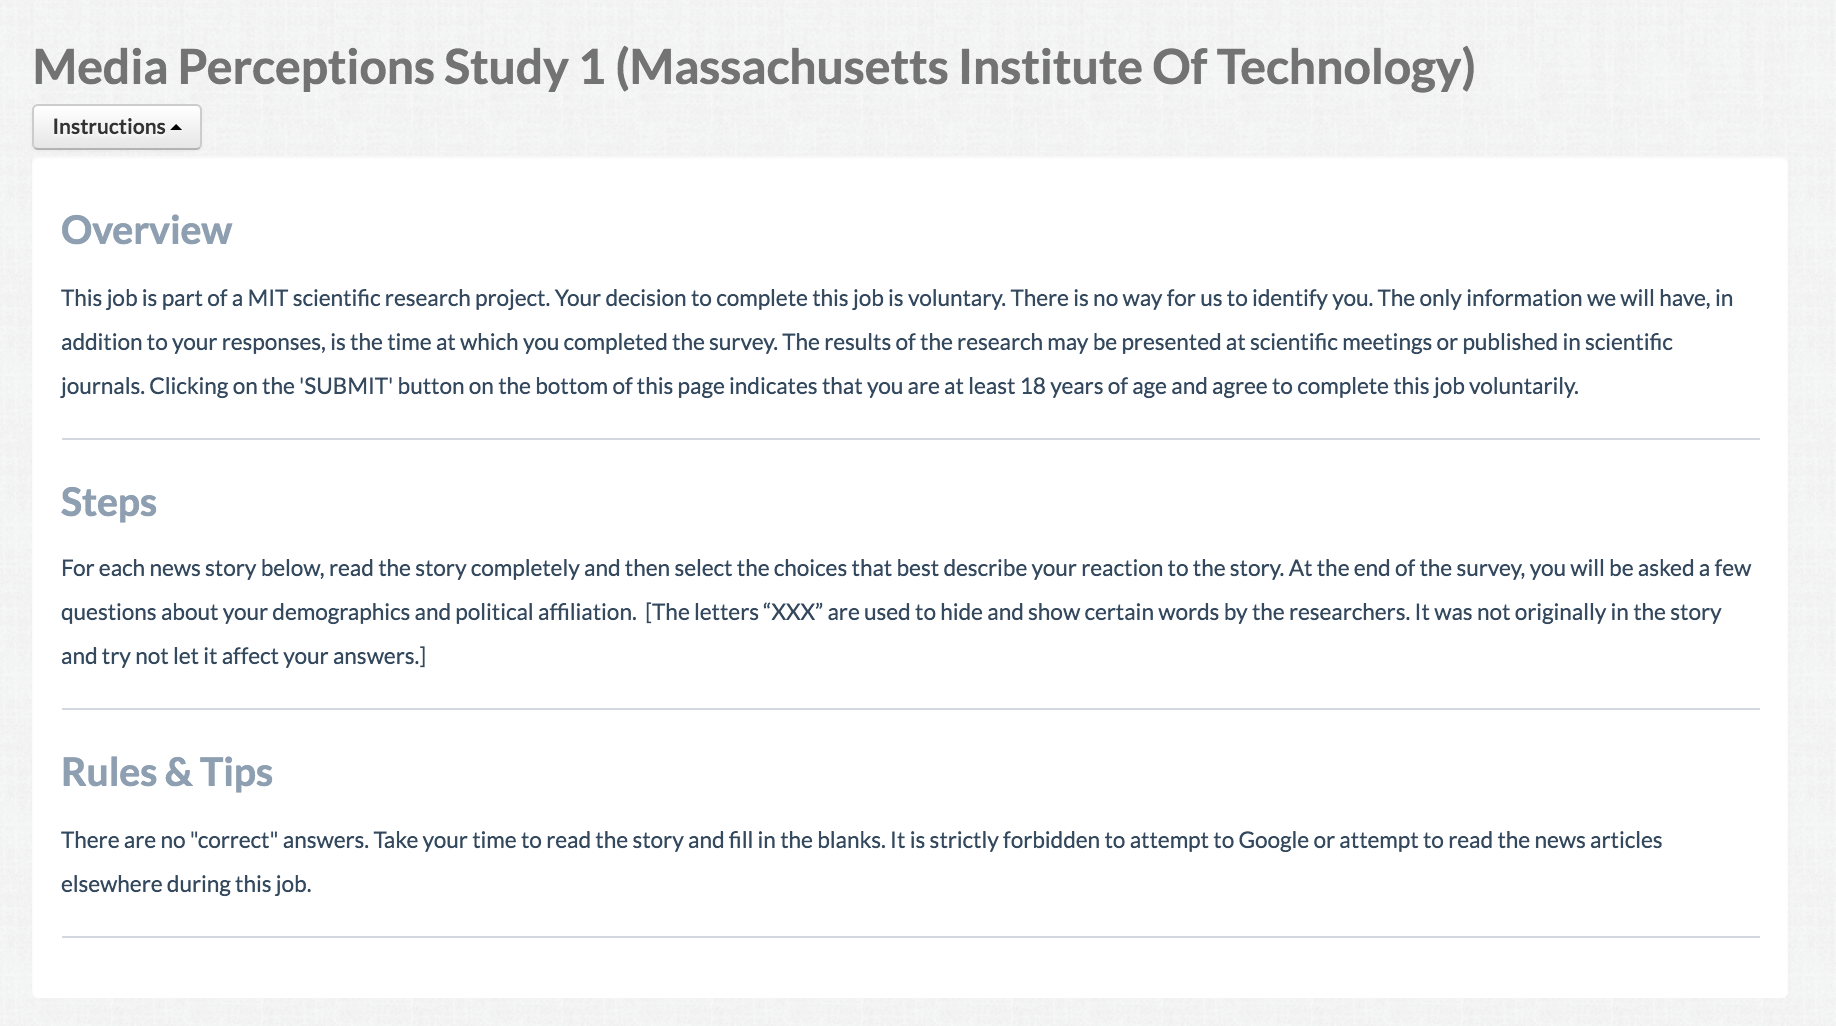
\includegraphics[width=\textwidth]{crowdflower_instructions}
 
\section{Demographic Survey}
\section{Political Affiliation Survey}
\section{Quality Assurance}
%-Filter by nationality
%- highest setting on crowdflower
%- Gold questions
%- time limits
%n- price